\section{Cassandra}
O Cassandra, com seu modelo híbrido chave-valor/relacional, facilita o desenvolvimento de certas aplicações.

\subsection{Modelo de Dados}
\begin{frame}{Apache Cassandra}
\begin{itemize}
\item Híbrido entre chave-valor e relacional
\item Valores, ou linhas, são agrupados em \emph{column families} (equivalente a tabelas)
\item Column Families, juntas formam um \emph{keyspace} (equivalente a um banco de dados)
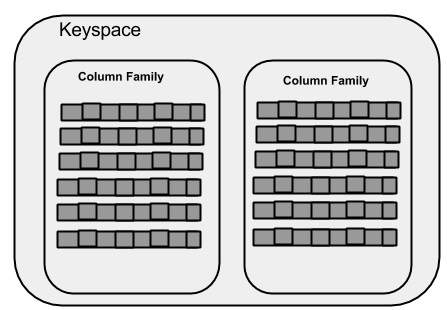
\includegraphics[width=.7\textwidth]{images/cass_keyspace}
\end{itemize}
\end{frame}


\begin{frame}{Apache Cassandra}
\begin{itemize}
\item Chave mapeia para um conjunto de colunas
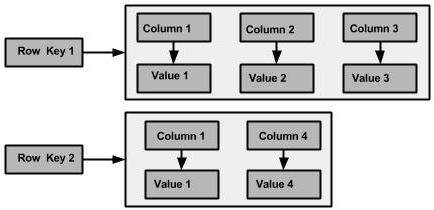
\includegraphics[width=.7\textwidth]{images/cass_column_family}

\item Cada coluna tem valor e timestamp
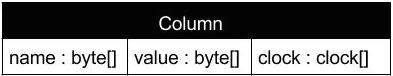
\includegraphics[width=.7\textwidth]{images/cass_column}


\item Linhas podem ser ordenadas por valores de algumas colunas (chave composta)

\item Colunas podem ser agrupadas em {\emph super-columns}\\
(Nao recomendado)

%\item \emph{Range Queries} -- todas a linhas com chave em determinada faixa de valores
\end{itemize}
\end{frame}




\begin{frame}[fragile,allowframebreaks]{Apache Cassandra}
\begin{itemize}
\item Super-column families

%\begin{verbatim}
%UserList={    <- Table (Tables pertencem a um keyspace)
%     Cath:{   <- Chave
%         //Super column
%         username:{firstname:”Cath”, lastname:”Yoon”}
%         address:{ city:”Seoul”,postcode:”1234”}}
%           
%     Terry:{   //Super columns formam super column families
%         //Columns formam column families.
%         username:{firstname:”Terry”,lastname:”Cho”}
%         account:{bank:”hana”,account:”1234”}}
%}
%\end{verbatim}

\item Cassandra Query Language
\end{itemize}

\url{http://wiki.apache.org/cassandra/FrontPage}
\end{frame}


\begin{frame}{Demo}
\url{https://blog.rackspace.com/cassandra-by-example}

\url{http://wiki.apache.org/cassandra/GettingStarted}	
\end{frame}

É possível rodar o Cassandra facilmente em certas nuvens computacionais.


\begin{frame}[allowframebreaks]{Amazon Web Services}
\begin{itemize}
\item Crie uma conta gratuita

\item Se você é estudante, registre-se no \href{https://www.awseducate.com/Registration}{AWS Educate} para mais opções.

\item Abra o \href{https://console.aws.amazon.com/console/home}{AWS Console}

\item Clique em \href{https://console.aws.amazon.com/ec2/}{EC2}

\item Clique em Launch Instance

\item Selecione Free Tier Only

\framebreak

\item Encontre uma Amazon Machine Image (AMI) basada em Ubuntu e clique em Select, na frente do nome.

\item Selecione t2.micro (free tier elegible)

\item Clique em Review and Launch

\item Clique em Launch

\item Selecione Create a new key pair

\item Dê um nome para seu par de chaves e salve-o em lugar seguro como chave.pem

\item Clique mais uma vez em Launch

\item Clique em View Instance

\item A partir do Console também pode ver suas instâncias clicando em \href{https://console.aws.amazon.com/ec2/v2/home?region=us-east-1\#Instances:}{Instances}
\end{itemize}
\end{frame}

\begin{frame}[fragile,allowframebreaks]{Conectando-se}
\begin{itemize}
	\item Ao selecionar uma instância, você pode ver seu nome na parte de baixo da tela. Por exemplo, \textbf{ec2-107-22-156-46.compute-1.amazonaws.com}
	
	\item chmo 400 chave.pem
	
	\item ssh -i chave.pem ubuntu@<endereco>
	
	\item siga as instruções \href{http://cassandra.apache.org/doc/latest/getting_started/installing.html#installation-from-debian-packages}{aqui}
	
	
	\item sudo service cassandra start
	\item nodetool status

	\begin{scriptsize}
\begin{verbatim}
Datacenter: datacenter1
=======================
Status=Up/Down
|/ State=Normal/Leaving/Joining/Moving
--  Address    Load       Tokens  Owns (effective) Host ID  Rack
UN  127.0.0.1  112.12 KiB  256    100.0%           xxx      rack1
\end{verbatim}	
	\end{scriptsize}
\end{itemize}
\end{frame}

\begin{frame}{Cassandra}
/etc/cassandra/cassandra.yaml
\end{frame}

\begin{frame}[allowframebreaks,fragile]{Dados}
Seguiremos o tutorial \href{https://www.tutorialspoint.com/cassandra/cassandra_create_keyspace.htm}{aqui}

\begin{verbatim}
cqlsh
	
cqlsh.> CREATE KEYSPACE tutorialspoint
WITH replication = {'class':'SimpleStrategy',
'replication_factor':1};
	
cqlsh> DESCRIBE keyspaces;


	\end{verbatim}
\end{frame}

Outra opcao seria o Network Topology Strategy, em que pode setar o numero de replicas por data-center

\begin{frame}[allowframebreaks,fragile]{Dados}
\begin{verbatim}
cqlsh> SELECT * FROM system.schema_keyspaces;

cqlsh> USE tutorialspoint;

CREATE TABLE emp(emp_id int PRIMARY KEY,
emp_name text,emp_city text,
emp_sal varint,emp_phone varint);











INSERT INTO 
emp (emp_id, emp_name, emp_city, emp_phone, emp_sal) VALUES(1,'ram', 'Hyderabad', 9848022338, 50000);

INSERT INTO 
emp (emp_id, emp_name, emp_city,emp_phone, emp_sal) 
VALUES(2,'robin', 'Hyderabad', 9848022339, 40000);

INSERT INTO 
emp (emp_id, emp_name, emp_city,emp_phone, emp_sal) 
VALUES(3,'rahman', 'Chennai', 9848022330, 45000);






select * from emp;
\end{verbatim}
\end{frame}



\begin{frame}{Multi-node}
\href{https://github.com/pcmanus/ccm}{Cassandra Cluster Management}

\begin{itemize}
	\item sudo apt install python-pip
	\item sudo pip install ccm
	\item sudo ifconfig lo0 alias 127.0.0.2 up
	\item sudo ifconfig lo0 alias 127.0.0.3 up	
	\item ccm create test -v 3.9
	\item ccm populate -n 3
	\item service cassandra stop (apt-get)
	\item vim .ccm/test/node1/conf/cassandra.yaml
	\item start\_rpc=true
	\item ccm start
	\item ccm info
	\item ccm node[1-3] show
	\item ccm
	\item cqlsh
\end{itemize}
\end{frame}

\begin{frame}{Falhas}

\begin{itemize}
	\item Insira dados no sistema, com fator de replicaç~ao 2
	\item Consulte os dados\\~\\~\\
	\item ps aux
	\item kill 9 PID
	\item Consulte os dados\\~\\~\\
\end{itemize}
\end{frame}
